%%%%%%%%%%%%%%%%%%%%%%%%%%%%%%%%%%%%%%%%%
% Beamer Presentation
% LaTeX Template
% Version 1.0 (10/11/12)
%
% This template has been downloaded from:
% http://www.LaTeXTemplates.com
%
% License:
% CC BY-NC-SA 3.0 (http://creativecommons.org/licenses/by-nc-sa/3.0/)
%
%%%%%%%%%%%%%%%%%%%%%%%%%%%%%%%%%%%%%%%%%

%----------------------------------------------------------------------------------------
%	PACKAGES AND THEMES
%----------------------------------------------------------------------------------------

\documentclass{beamer}
\usepackage{color}
\definecolor{green}{HTML}{4CAF50}

\mode<presentation> {

% The Beamer class comes with a number of default slide themes
% which change the colors and layouts of slides. Below this is a list
% of all the themes, uncomment each in turn to see what they look like.

\usetheme{default}
 %\usetheme{AnnArbor}
%\usetheme{Antibes}
%\usetheme{Bergen}
%\usetheme{Berkeley}
 %\usetheme{Berlin}
 %\usetheme{Boadilla}
%\usetheme{CambridgeUS}
%\usetheme{Copenhagen}
%\usetheme{Darmstadt}
%\usetheme{Dresden}
%\usetheme{Frankfurt}
%\usetheme{Goettingen}
%\usetheme{Hannover}
%\usetheme{Ilmenau}
%\usetheme{JuanLesPins}
%\usetheme{Luebeck}
%\usetheme{Madrid}
%\usetheme{Malmoe}
%\usetheme{Marburg}
%\usetheme{Montpellier}
%\usetheme{PaloAlto}
%\usetheme{Pittsburgh}
%\usetheme{Rochester}
 %\usetheme{Singapore}
%\usetheme{Szeged}
 %\usetheme{Warsaw}

% As well as themes, the Beamer class has a number of color themes
% for any slide theme. Uncomment each of these in turn to see how it
% changes the colors of your current slide theme.
%\usecolortheme{albatross}
%\usecolortheme{beaver}
%\usecolortheme{beetle}
%\usecolortheme{crane}
%\usecolortheme{dolphin}
%\usecolortheme{dove}
%\usecolortheme{fly}
%\usecolortheme{lily}
%\usecolortheme{orchid}
%\usecolortheme{rose}
%\usecolortheme{seahorse}
%\usecolortheme{whale}
 \setbeamercolor*{palette primary}{use=structure,fg=white,bg=green}
 \setbeamercolor*{palette secondary}{use=structure,fg=white,bg=green}
 \setbeamercolor*{palette tertiary}{use=structure,fg=white,bg=green}
  \setbeamercolor{title}{fg=white,bg=green}
 \setbeamercolor{frametitle}{fg=white,bg=green}
  \setbeamercolor{block title}{fg=white,bg=green}
\setbeamercolor{item}{fg=green}

%\setbeamertemplate{footline} % To remove the footer line in all slides uncomment this line
%\setbeamertemplate{footline}[page number] % To replace the footer line in all slides with a simple slide count uncomment this line

%\setbeamertemplate{navigation symbols}{} % To remove the navigation symbols from the bottom of all slides uncomment this line
}

\usepackage{graphicx} % Allows including images
\usepackage{booktabs} % Allows the use of \toprule, \midrule and \bottomrule in tables
\usepackage{pgfgantt}
%----------------------------------------------------------------------------------------
%	TITLE PAGE
%----------------------------------------------------------------------------------------

\title[ROPE09]{ROPE09: No likey, no lighty!} % The short title appears at the bottom of every slide, the full title is only on the title page

\author{Paul McGurk\\\medskip \footnotesize{Advisor: Dr Marc Roper\\
Second Marker: Dr Mark Dukes}} % Your name
\institute[University of Strathclyde] % Your institution as it will appear on the bottom of every slide, may be shorthand to save space
{
University of Strathclyde \\ % Your institution for the title page
\medskip
\textit{paul@mcgurk.co\\} % Your email address
}
\date{December 9, 2015} % Date, can be changed to a custom date

\begin{document}

\begin{frame}
\titlepage % Print the title page as the first slide
\end{frame}

%----------------------------------------------------------------------------------------
%	PRESENTATION SLIDES
%----------------------------------------------------------------------------------------

\section{Project Aims and Objectives}
\begin{frame}
\subsection{Project Aims}
\frametitle{Project Aims and Objectives}
\begin{block}{Aims}
\begin{enumerate}
	\item Overcome the problems with traditional classroom clickers, i.e. Expensive, dedicated hardware, impractical for large classes.
	\item Ability to be used to guage the current feeling in the class.
	\item Allow Lecturers to tailor their lectures based on responses.
\end{enumerate}
\end{block}
\subsection{Project Objectives}
\begin{block}{Objectives}
  \begin{itemize}
	\item Peer to Peer network through Wi-Fi direct.
	\item Interface with ``Lecturer'' and ``Student'' versions.
	\item Ability to set/ questions on ``Lecturer'/''Student''' account.
	\item Use of some sort of display to display feedback.
	\item Ability to access interface through various devices.
	\item Display feedback data in a simplified way, possibly through a Dotti.
\end{itemize}
\end{block}
\end{frame}

\section{Progress}
\begin{frame}
\frametitle{Progress}
\subsection{Background Research}
\begin{block}{Background Research}
There is a number of similar devices out there. Most suffer from the issues that inspired this project, such as expensive licenses and lots of dedicated hardware. 
\end{block}
\begin{block}{Requirements}
\begin{enumerate}
	\item Cheap, portable and easy to use.
	\item Interface with ``Lecturer'' and ``Student'' versions.
	\item Ability to set/ questions on ``Lecturer'/''Student''' account.
	\item Use of some sort of display to display feedback.
	\item Ability to access interface through various devices.
\end{enumerate}
\end{block}
\end{frame}


\begin{frame}
\frametitle{Progress}
\begin{columns}[c] % The "c" option specifies centered vertical alignment while the "t" option is used for top vertical alignment

\column{.75\textwidth} % Right column and width
\begin{block}{Web Application}
The initial framework of the web application has been set up using Materialize, a JavaScript/CSS library that follows Google's material design. In addition, a mock version of the Student's interface was created, with a hardcoded question to get the design of the interface ready for full implementation.\\
\end{block}
\medskip
    \tiny{\centering{Userflow}}\\
    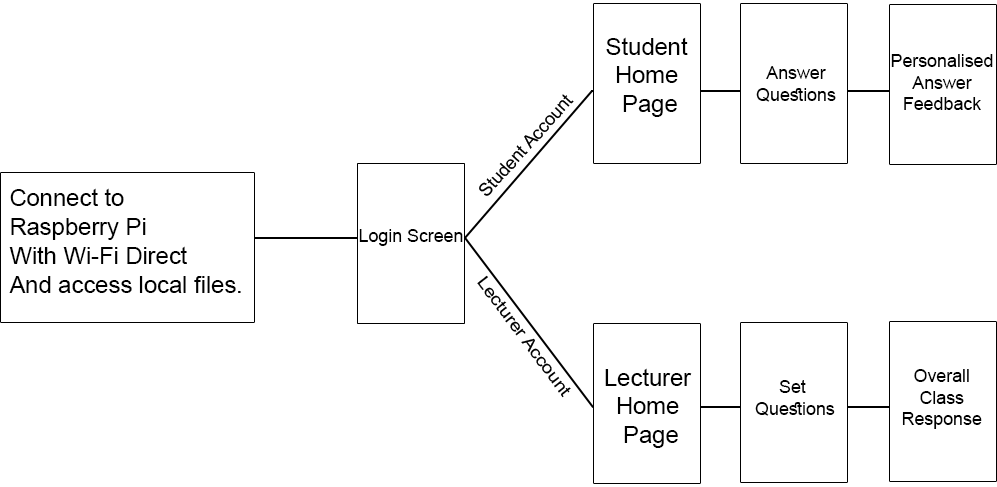
\includegraphics[width=0.75\textwidth]{userflow.png}\\
\column{.25\textwidth} % Left column and width
    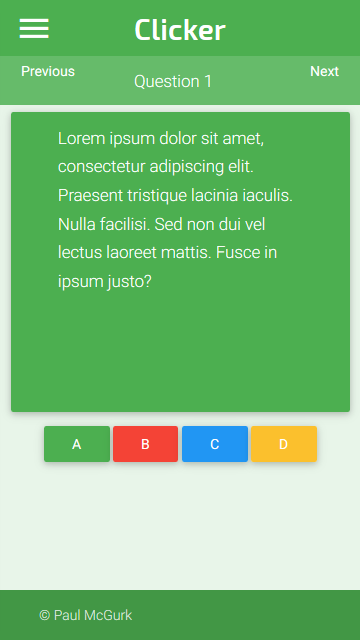
\includegraphics[height=5cm]{studentinterface.png}\\
    \tiny{\centering{a mock question on the student interface}}
\end{columns}
\end{frame}

\begin{frame}
\frametitle{Progress}
\subsection{Communication}
\begin{block}{Communication}
Communication between a Raspberry Pi with a WiFi antenna, and a Mobile Phone (Nexus 5X, Android 6.0), has been achieved, but is still at an early stage. Wi-Fi direct is more complex than initially figured, and will require more investigation to know if it is capable of being implemented in a way that is useful to this project.\\
In response to the risk of Wi-Fi direct not having the capabilities required, a number of alternatives have been derived, such as:
\begin{enumerate}
	\item Using the Raspberry Pi as a Wi-Fi access point to access the local Web server.
	\item Taking the Raspberry Pi out of the equation, and using a remote Web server for the Web application.
\end{enumerate}
These alternatives do not affect the development of the web application as planned.
\end{block}
\end{frame}
%------------------------------------------------
\section{Technology Used} % Sections can be created in order to organize your presentation into discrete blocks, all sections and subsections are automatically printed in the table of contents as an overview of the talk
%------------------------------------------------

 % A subsection can be created just before a set of slides with a common theme to further break down your presentation into chunks

\subsection{Technology Overview}
\begin{frame}
\frametitle{Technology Overview}
\begin{block}{Web Application}
The web application will be implemented in a mixture of HTML5, CSS3 for the GUI, JavaScript for the client based functionality, PHP for the client to server communication and MySQL for the database functionality.
\end{block}

\begin{block}{Web Host}
The web host is a Raspberry Pi that will be located within the classroom. Wi-Fi direct devices will then connect to this Pi and access it's local web pages, as well as a MySQL database.
\end{block}

\begin{block}{Communication}
Communication will be achieved through the use of Wi-Fi direct. Wi-Fi direct is a Wi-Fi standard that enables devices to connect and communicate without using a wireless access point. It communicates with more than one device simultaneously at Wi-Fi speeds.
\end{block}
\end{frame}

\subsection{Technology Stack Diagram}
\begin{frame}
\frametitle{Technology Stack Diagram}
\begin{centering}
    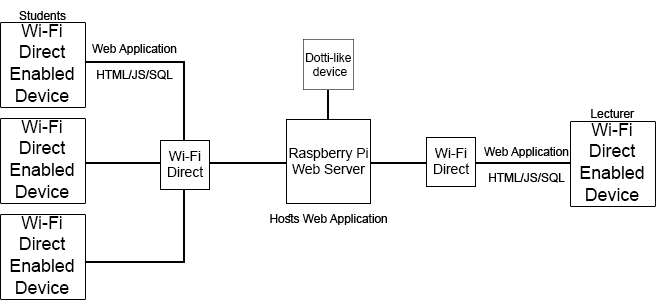
\includegraphics[width=1\textwidth]{stackdiagram.png}
\end{centering}
\end{frame}

%------------------------------------------------

\section{Evaluation}
\subsection{Evaluation}
\begin{frame}
\frametitle{Evaluation}
\begin{block}{Target Users}
Target users will be a mix of both Students and Lecturers.
\end{block}

\begin{block}{Method}
Evaluation will involve a live preview of the system in the intended environment with the target end users; a lecturer and students. These users will be recruited by contacting lecturers and inquiring if it would be a system they would be interested in, with students in the class optionally choosing to use the system within the setting or not.

Participants will be expected to simply use the system in place of a normal class-room clicker, with questions being set by the lecturer and the students answering them on their Wi-Fi direct enabled devices. \\

\end{block}

\end{frame}

\begin{frame}
\section{Schedule}
\frametitle{Schedule}
\begin{centering}
    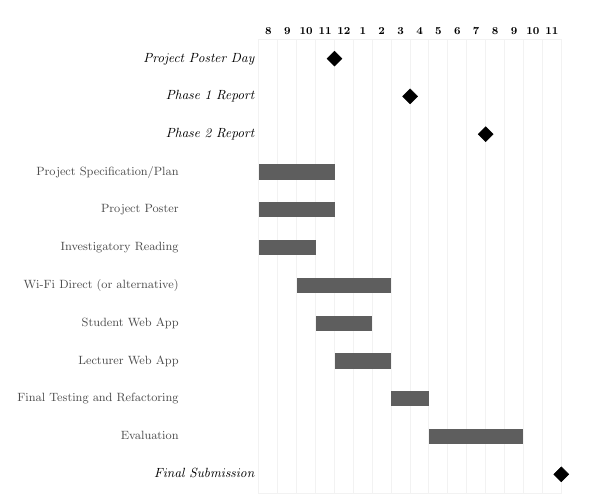
\includegraphics[width=0.7\textwidth]{schedule.png}
\end{centering}
\end{frame}


\begin{frame}
\Huge{\centerline{The End}}
\end{frame}

%----------------------------------------------------------------------------------------

\end{document} 